\documentclass[12pt]{article}
\usepackage{amsmath,amsthm}
\usepackage{titlesec}
\usepackage{graphicx}
\usepackage{longtable}
\usepackage{array}
\usepackage{hyperref}

\newtheorem{lemma}{Lemma}
\newtheorem{theorem}{Theorem}
\titleformat{\section}
{\normalfont\Large\bfseries}{Question~\thesection:}{1em}{}
\newlength{\toppush}
\setlength{\toppush}{2\headheight}
\addtolength{\toppush}{\headsep}
\def\subjnum{CS120}
\def\subjname{Web Programming and Engineering}

\def\doheading#1#2#3{\vfill\eject\vspace*{-\toppush}%
  \vbox{\hbox to\textwidth{{\bf} \subjnum: \subjname \hfil Kevin Covney}%
    \hbox to\textwidth{{\bf} Tufts University, Summer 2026 \hfil#3\strut}%
    \hrule}}

\newcommand{\htitle}[1]{\vspace*{1.25ex plus 1ex minus 0ex}%
\begin{center}
{\large\bf #1}
\end{center}} 


%%%%%%%%%%%%%%%%%%%%%%%%%%%%%%%%%%%%%%%%%%%%%%%%%%%%%%%%%%%%%%%%%%%
% BEGIN DOCUMENT
%%%%%%%%%%%%%%%%%%%%%%%%%%%%%%%%%%%%%%%%%%%%%%%%%%%%%%%%%%%%%%%%%%%
\begin{document}
\doheading{2}{title}{Assignment 3: CSS}
\section*{Links}

\noindent URL of me\_two.html: \url{https://kcovney.github.io/hw2-3/me_two.html}

\section*{Design}

The purpose of this website is to advertise the Detroit-based guitar duo Super Guitar Bros. They primarily make money through

\begin{enumerate}
    \item Ticket sales, either on tour or on one-off shows
    \item Google AdSense via their YouTube channel
    \item Streaming on various streaming platforms—primarily YouTube Music, Apple Music, Spotify
    \item Their Patreon account, where patrons can donate a set amount of money each month to get access to premium content
\end{enumerate}

Their goal is primarily to gain more active listeners and patrons and to bring people to their shows. The users are primarily listeners, and potentially also booking managers who want to see if Super Guitar Bros. would be a good fit for their concert venue. The user's goal would be to view their tour dates, buy their merch, or see where they can listen to the band. In order for the site to be effective, it has to display the relevant information in a way that's legible and also advertise their personality and showcase what makes them special as a musical group.

The site navigation will have a clean layout, with tour dates front and center, as well as embedded YouTube videos, links to their YouTube channel, Patreon, merch store, and their pages on various streaming platforms. It will also feature photos of them. \vspace{1em}

The Super Guitar Bros. gained a following in the early days of YouTube playing guitar covers of popular video game compositions, TV themes, and movie music. As such, the website will have a vintage, Nintendo-coded design with vibrant colors, unapologetically 3D graphics, and a retro aesthetic. It will be just as cool as they are. One important consideration is that, given Nintendo is an especially litigious company that protects their IP, none of the elements should be explicitly borrowing from Nintendo. 

\pagebreak

\section*{Navigation}

The top of the website will be a fixed-position navbar with a dropdown menu to listen to them on streaming platforms, a button that redirects to their pre-existing merch store, and a dropdown menu to watch their videos and view their social media accounts.

Under the navbar will be their logo with a background photo of them that should communicate their vibe.

Given their revenue streams, front and center on the home page and below the navbar and logo/photo will be their upcoming performances with dates, times, locations, and links to purchase tickets. Under that will be embedded YouTube videos, and below that, potentially some links to streaming services.

At the bottom will be a handful of lesser links to various other resources, such as copyright, privacy, terms of use, cookie settings, and the like. 

\pagebreak

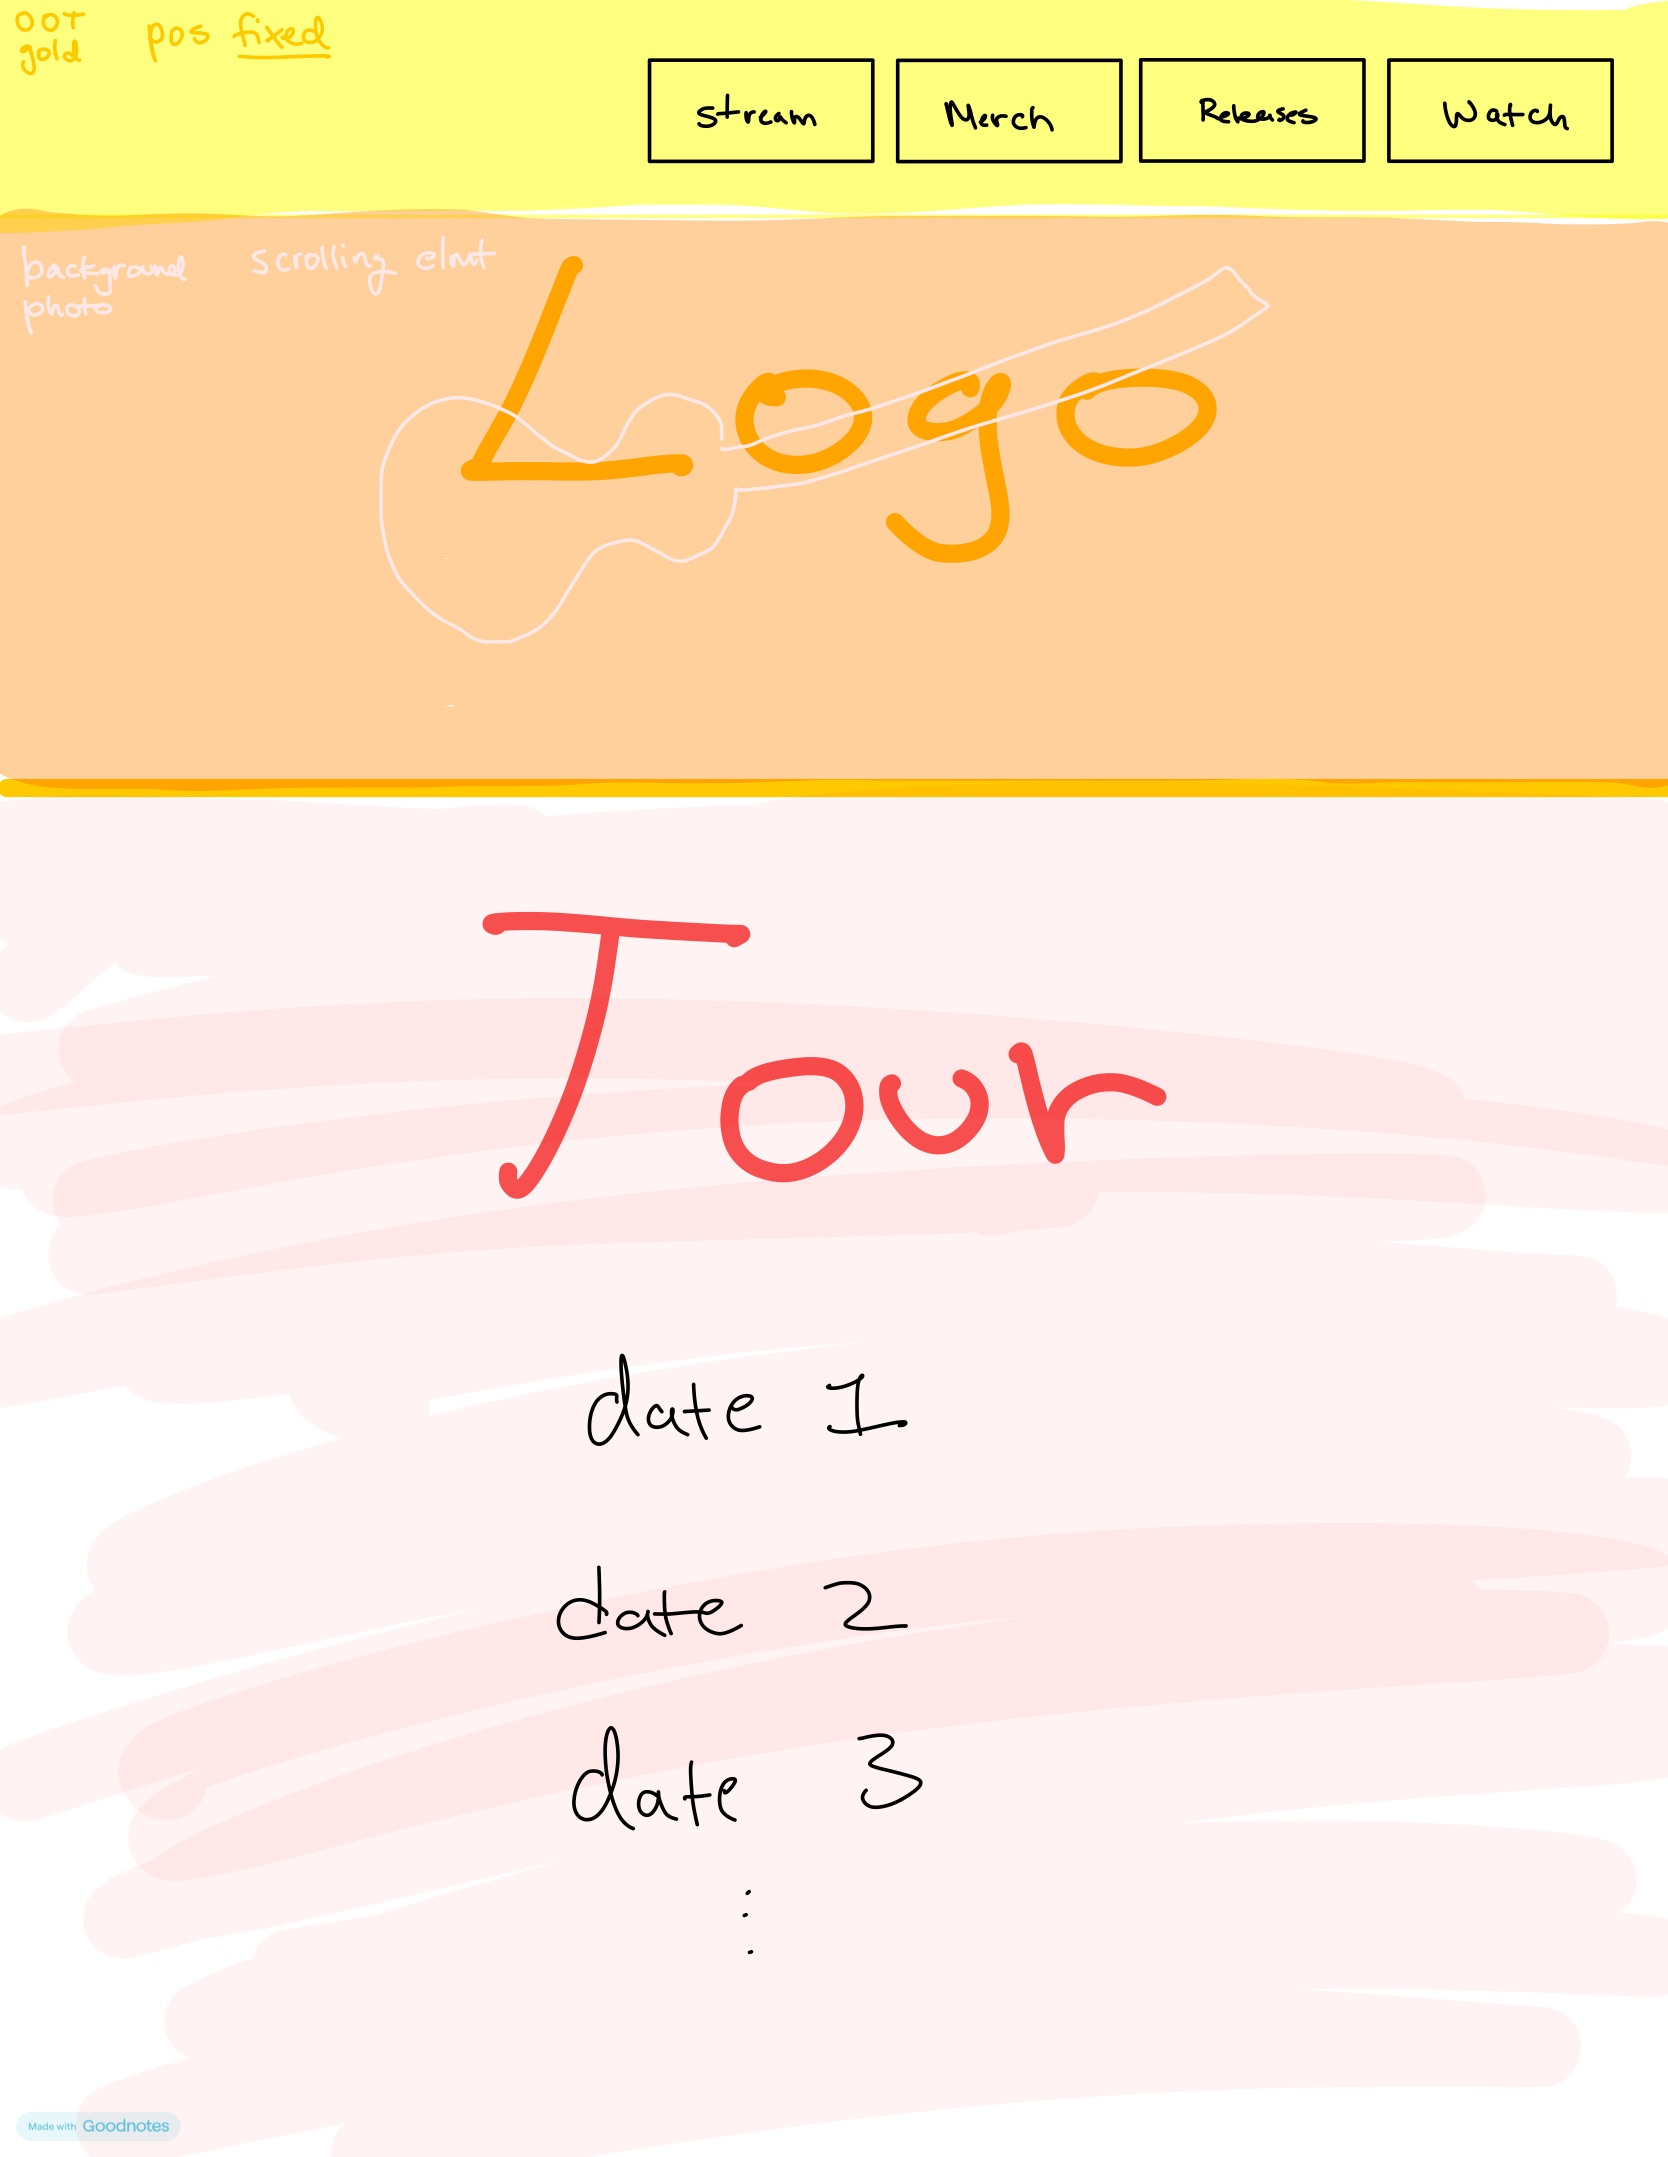
\includegraphics[width=0.8\textwidth]{band_site_homepage.jpg}

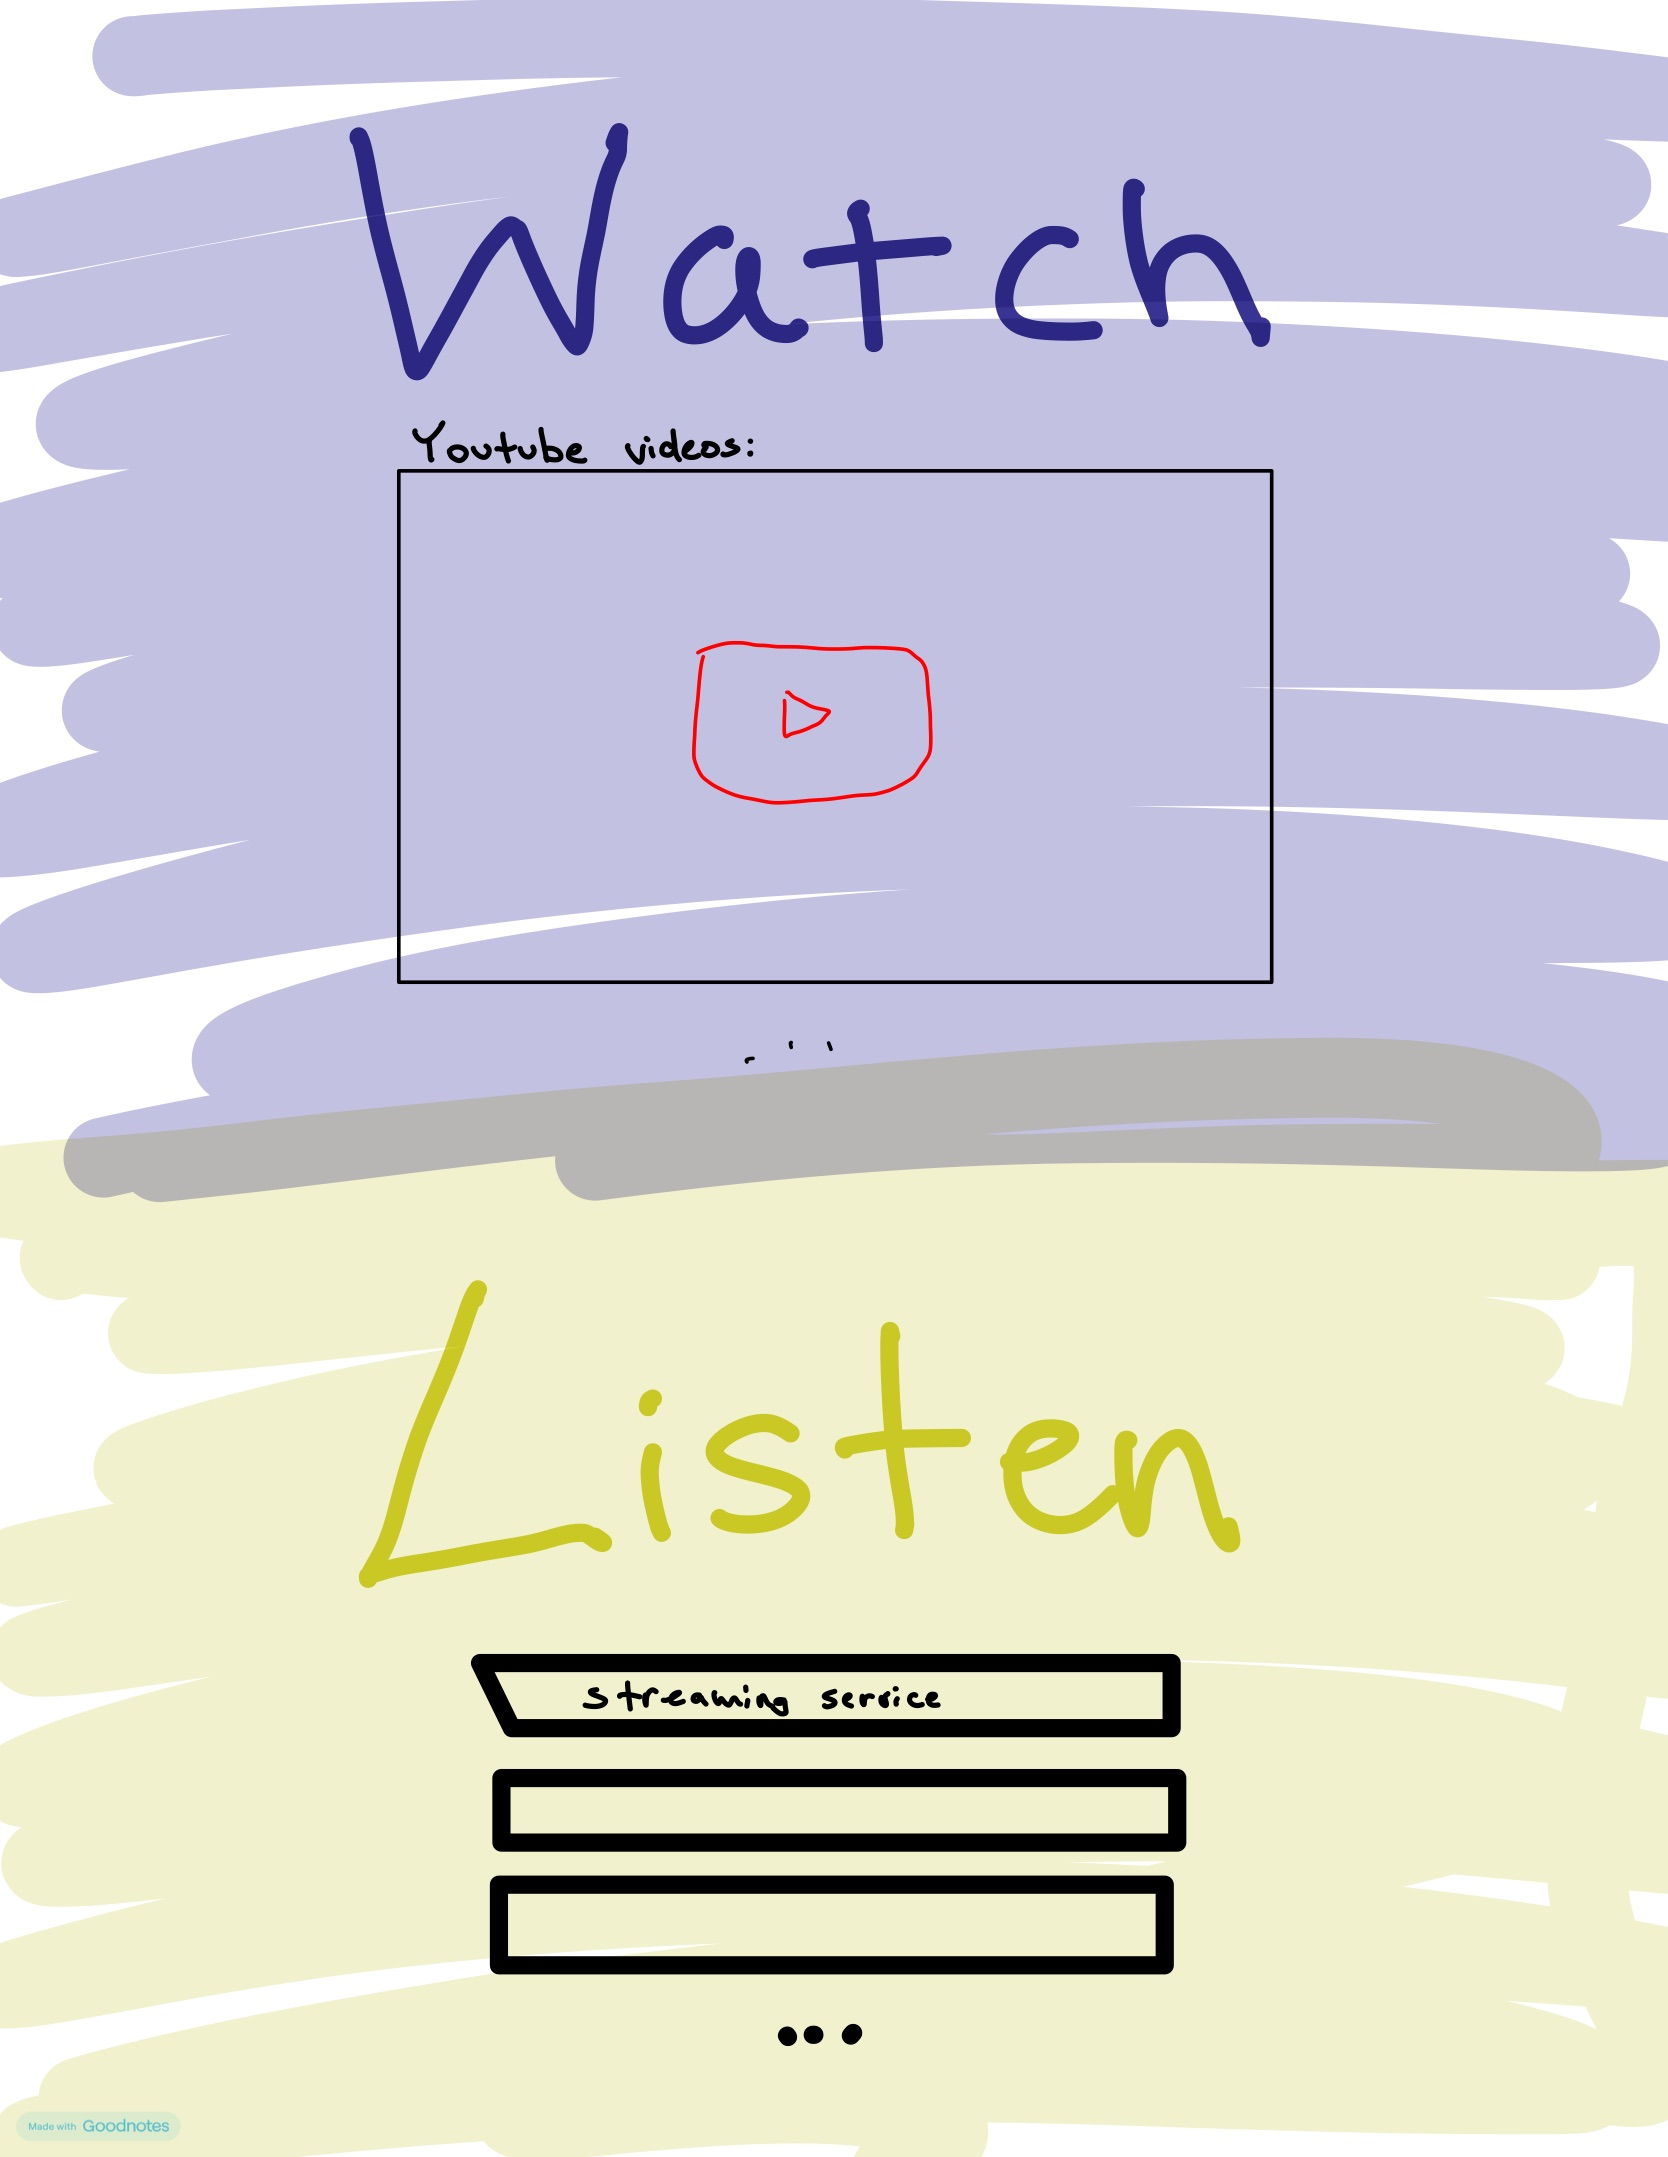
\includegraphics[width=0.8\textwidth]{band_site_homepage2.jpg}

\pagebreak

\section*{Homepage Content}

\setlength{\arrayrulewidth}{0.4mm}
\setlength{\tabcolsep}{64pt}
\renewcommand{\arraystretch}{1.6}
\begin{tabular}{ |p{10cm}|  }
\hline
(Hero section) Title: Super Guitar Bros: The Duo Making Legendary Game Music \\
Fixed navbar: \hfill \fbox{Stream} \fbox{Store} \fbox{Watch} \\
\begin{center}
Logo and background photo \\
Two Guitars. Infinite Power-Ups.
\end{center} \\
\hline
(Tour Section)
Tour | Catch us in a city near you! \\ 
June 17 - Rec Room - Buffalo, NY \hfill \fbox{Tickets} \\
June 18 - Assembly - Kingston, NY \hfill \fbox{Tickets} \\
June 19 - House of Music - Portland, ME \hfill \fbox{Tickets} \\
\hline
(Video Section)
\begin{center}
Watch \\ 
Video: Zelda Ocarina of Time \\
Video: Donkey Kong Country - Aquatic Ambience
\end{center} \\
\hline
(Listening Section)
\begin{center}
Listen \\ Spotify \\ YouTube Music \\ Apple Music
\end{center} \\
\hline
(Footer) Super Guitar Bros | Detroit, MI
\begin{center}
Socials | Help | Cookie Settings | Contact
\end{center} \\
\hline
\end{tabular}

\end{document}
